\subsection{Reference Model: Second Order System}

In this report we will consider the \LEGOMOTOR{} as a black-box system for which the inner structure its unknown, thus our aim will be that of identifying its frequency response.

Generally speaking, the behaviour of a motor can be generalized quite well using a Second Order System [SOS] model with a pole in $0$, related to the step input function, and two complex conjugates roots with negative real part as a consequence of the BIBO stability of the system. 

Note that the \LEGOMOTOR{} may, or may not, contain inner circuits, possibly with a simple feedback mechanism, that transforms the input signal given to the motor with the aim - for example - to force the system to behave much more like a First Order System [FOS].

The transfer function of a Second Order System has the following general formulation:
\begin{equation}
  Y(s) = {{k \over {{s^2 \over {{\omega_n}^2}} + {2s{\xi} \over
        {\omega_n}} + 1}}U\left (s\right )}
\end{equation}\label{eq:responseSOS}

where $k$ is the gain, $\xi$ is the damping factor and $\omega_n$ stands for the the natural pulsation of the system. The SOS response to an input step function in the time domain can be appreciated in figure \ref{fig:responseSOS}. 

The output is characterized by an initial ramp, ending with the overshoot, followed by a damped oscillation that stabilizes to the so called \textit{steady state value} after a time $t_s$, known as \textit{settling time}, with a percentile error lower than a chosen factor $\alpha{}$.

\begin{figure}[htbp]
  \begin{center}
  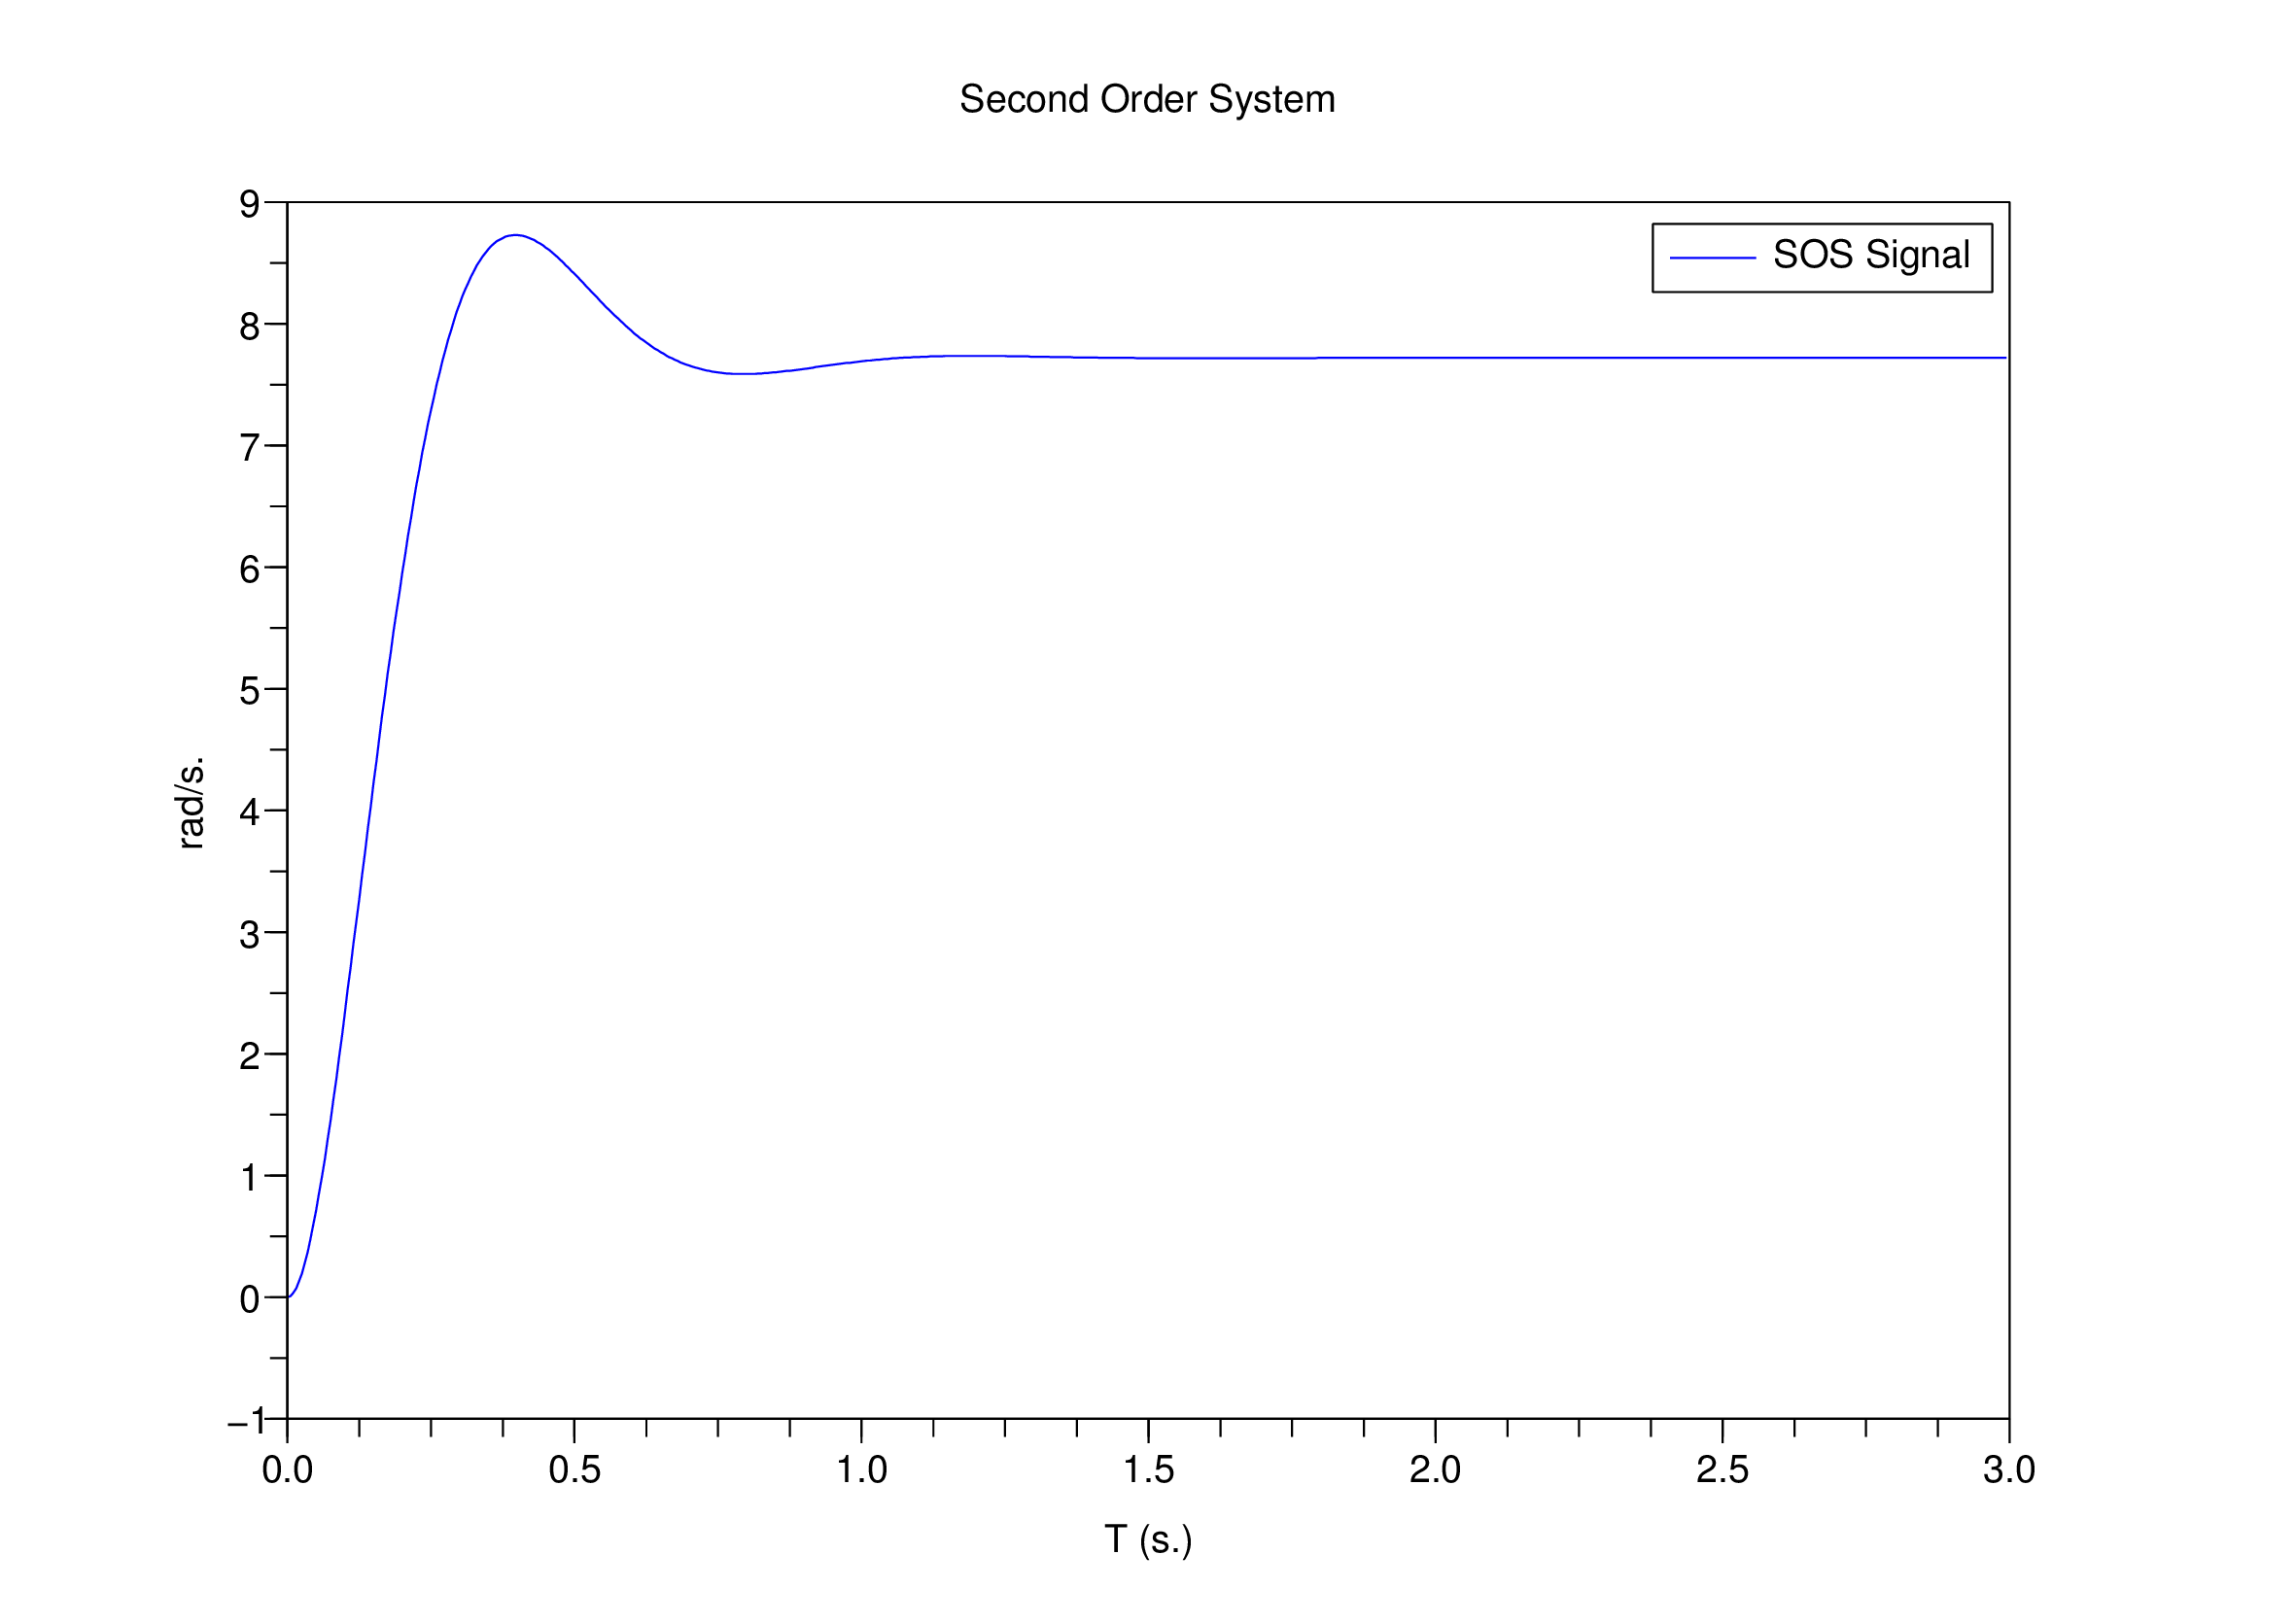
\includegraphics[scale=0.16]{FIGURES_1/Second_Order_System.png}
    \caption[SOS Response]{an example of time domain SOS response to an input step function, with $k: 1.7023353, \xi{}: 0.5570852, \omega_n{}: 14.139542$;}
    \label{fig:responseSOS}
  \end{center}
\end{figure}


%\newpage
\subsection{Experiment: Input Step Function}

In this experiment an input step function is fed to the \LEGOMOTOR{} and its response is evaluated in the \textit{time domain}. The goal of the experiment is to estimate the parameters characterizing the \LEGOMOTOR{} from the filtered speed response of the system, assuming a Second Order System reference model.

\subsubsection{Preparation of a new software platform}

Before doing any real experiment we rewrote from scratch the \textit{BRO\_{}spam\_{}client} sources so that:

\begin{itemize}
	\item The input function (step or sinusoidal) now is hard coded in to the Brick, relieving us from the need of exchanging control packets with the PC;
	\item The Brick's clock now can be used to have a better estimation of the time at which the samples are taken;
	\item There is a new definition of the bluetooth packets exchanged, which now encloses five fields: clock\_{}time, space, target\_{}power, target\_{}omega, is\_valid\_{}data. The packets are buffered before being sent out;
	\item Now the time interval of sampling can be safely lowered up to 2 milliseconds. Various tests at $2$, $5$ and $10$ millisecond[ms] have been conducted to ensure that these options worked. This allows more precise estimation of the response of the system. (As a side note, observe that to not loose bluetooth packets or get corrupted data smaller dimensions of the buffer must be preferred (5, 10) and it does help moving away from an environment that is noisy in the bluetooth or 802.11/b/g spectrum);
	\item Now the brick can be instructed to coordinate independently its own execution and collect an arbitrary number of experiments with user-defined options without the aid of human interaction; 
\end{itemize}

The \textit{BRO\_{}fist} and \textit{BRO\_{}comm} sources have been modified as well so that the data is printed on \textit{stderr} (which can be easily redirected to a file) instead of being sent to the \textit{Scilab} application.

\subsubsection{Measurements}

Initially we tried to sample our data with $2$ ms of sampling interval, however after some time we realized that the data was so oversampled that we were forced to proportionally redistribute the space covered during an interval of time even when the input step function did not have a so low power value.

Therefore, in the main experiment, we decided to fix our sampling interval to $5$ ms and to feed the motor with an input step function with power ranging from $10\%$ up to $100\%$ at intervals of $5\%$. For each power we produced $50$ tests, obtaining enough data for the next step of the identification procedure. All these tests have been made with the engine brake mode on.

\subsubsection{Data Loading and Filtering}

This phase has the goal to produce a filtered version of the speed response of the system that reassembles our target SOS model.

Once the file containing the data of a test is loaded, the vector of space is transformed into radians. The second step is to proportionally redistribute the covered space, if necessary, when an over-sampling phenomena occurs. This happens mostly when the sampling interval is low in respect to the capacity of the motor to rotate enough so that the Brick can detect this change. In such cases, omitting this step would give the wrong perception that the motor continuously switches from stationary periods to active states with a high instantaneous acceleration and an enormous speed. However we know by construction of the experiment that, excluding the initial adjustment time, the acceleration should be $0$ and the velocity constant.

The next step is the computation of the \textit{instantaneous speed} [IS] of the motor (\emph{first derivative}) using the collected data:
\[
  \omega(t) = {\Delta_\theta \over \Delta_t}
\]

The IS is still raw and characterized by errors due to the quantization, sampling and noise effect. Therefore we need to apply a \textit{low-pass filter} to eliminate the high frequencies.

We tried four different filters:
\begin{itemize}
\item \textbf{Moving Average Filter}, both simple and weighted, with a variable window with size ranging from $10$ up to $50$ samples;
\item \textbf{Exponential Filter} with a single \textit{forgetting factor} ranging from $0.05$ to $0.4$;
\item \textbf{Double Exponential Filter} with a couple of \textit{forgetting factors}, ranging again in the same discrete set of values;
\item \textbf{Butterworth Filter}, with an order of $3$ and various cut-off frequency values;
\end{itemize}

The first three operators produced a filtered signal that reassembled more the shape of a smoothed step with a high degree of noise rather than our target SOS model. The \textbf{butterworth} filter instead, designed to have a frequency response in the pass-band as flat as possible, revealed itself to produce a good filtered signal for our target SOS model. The only problem of this filter is that it introduces some delay, so that both the ramp and the over-shoot appear shifted in time, as shown in figure \ref{fig:butterworthResult}.

\begin{figure}[htbp]
\center
  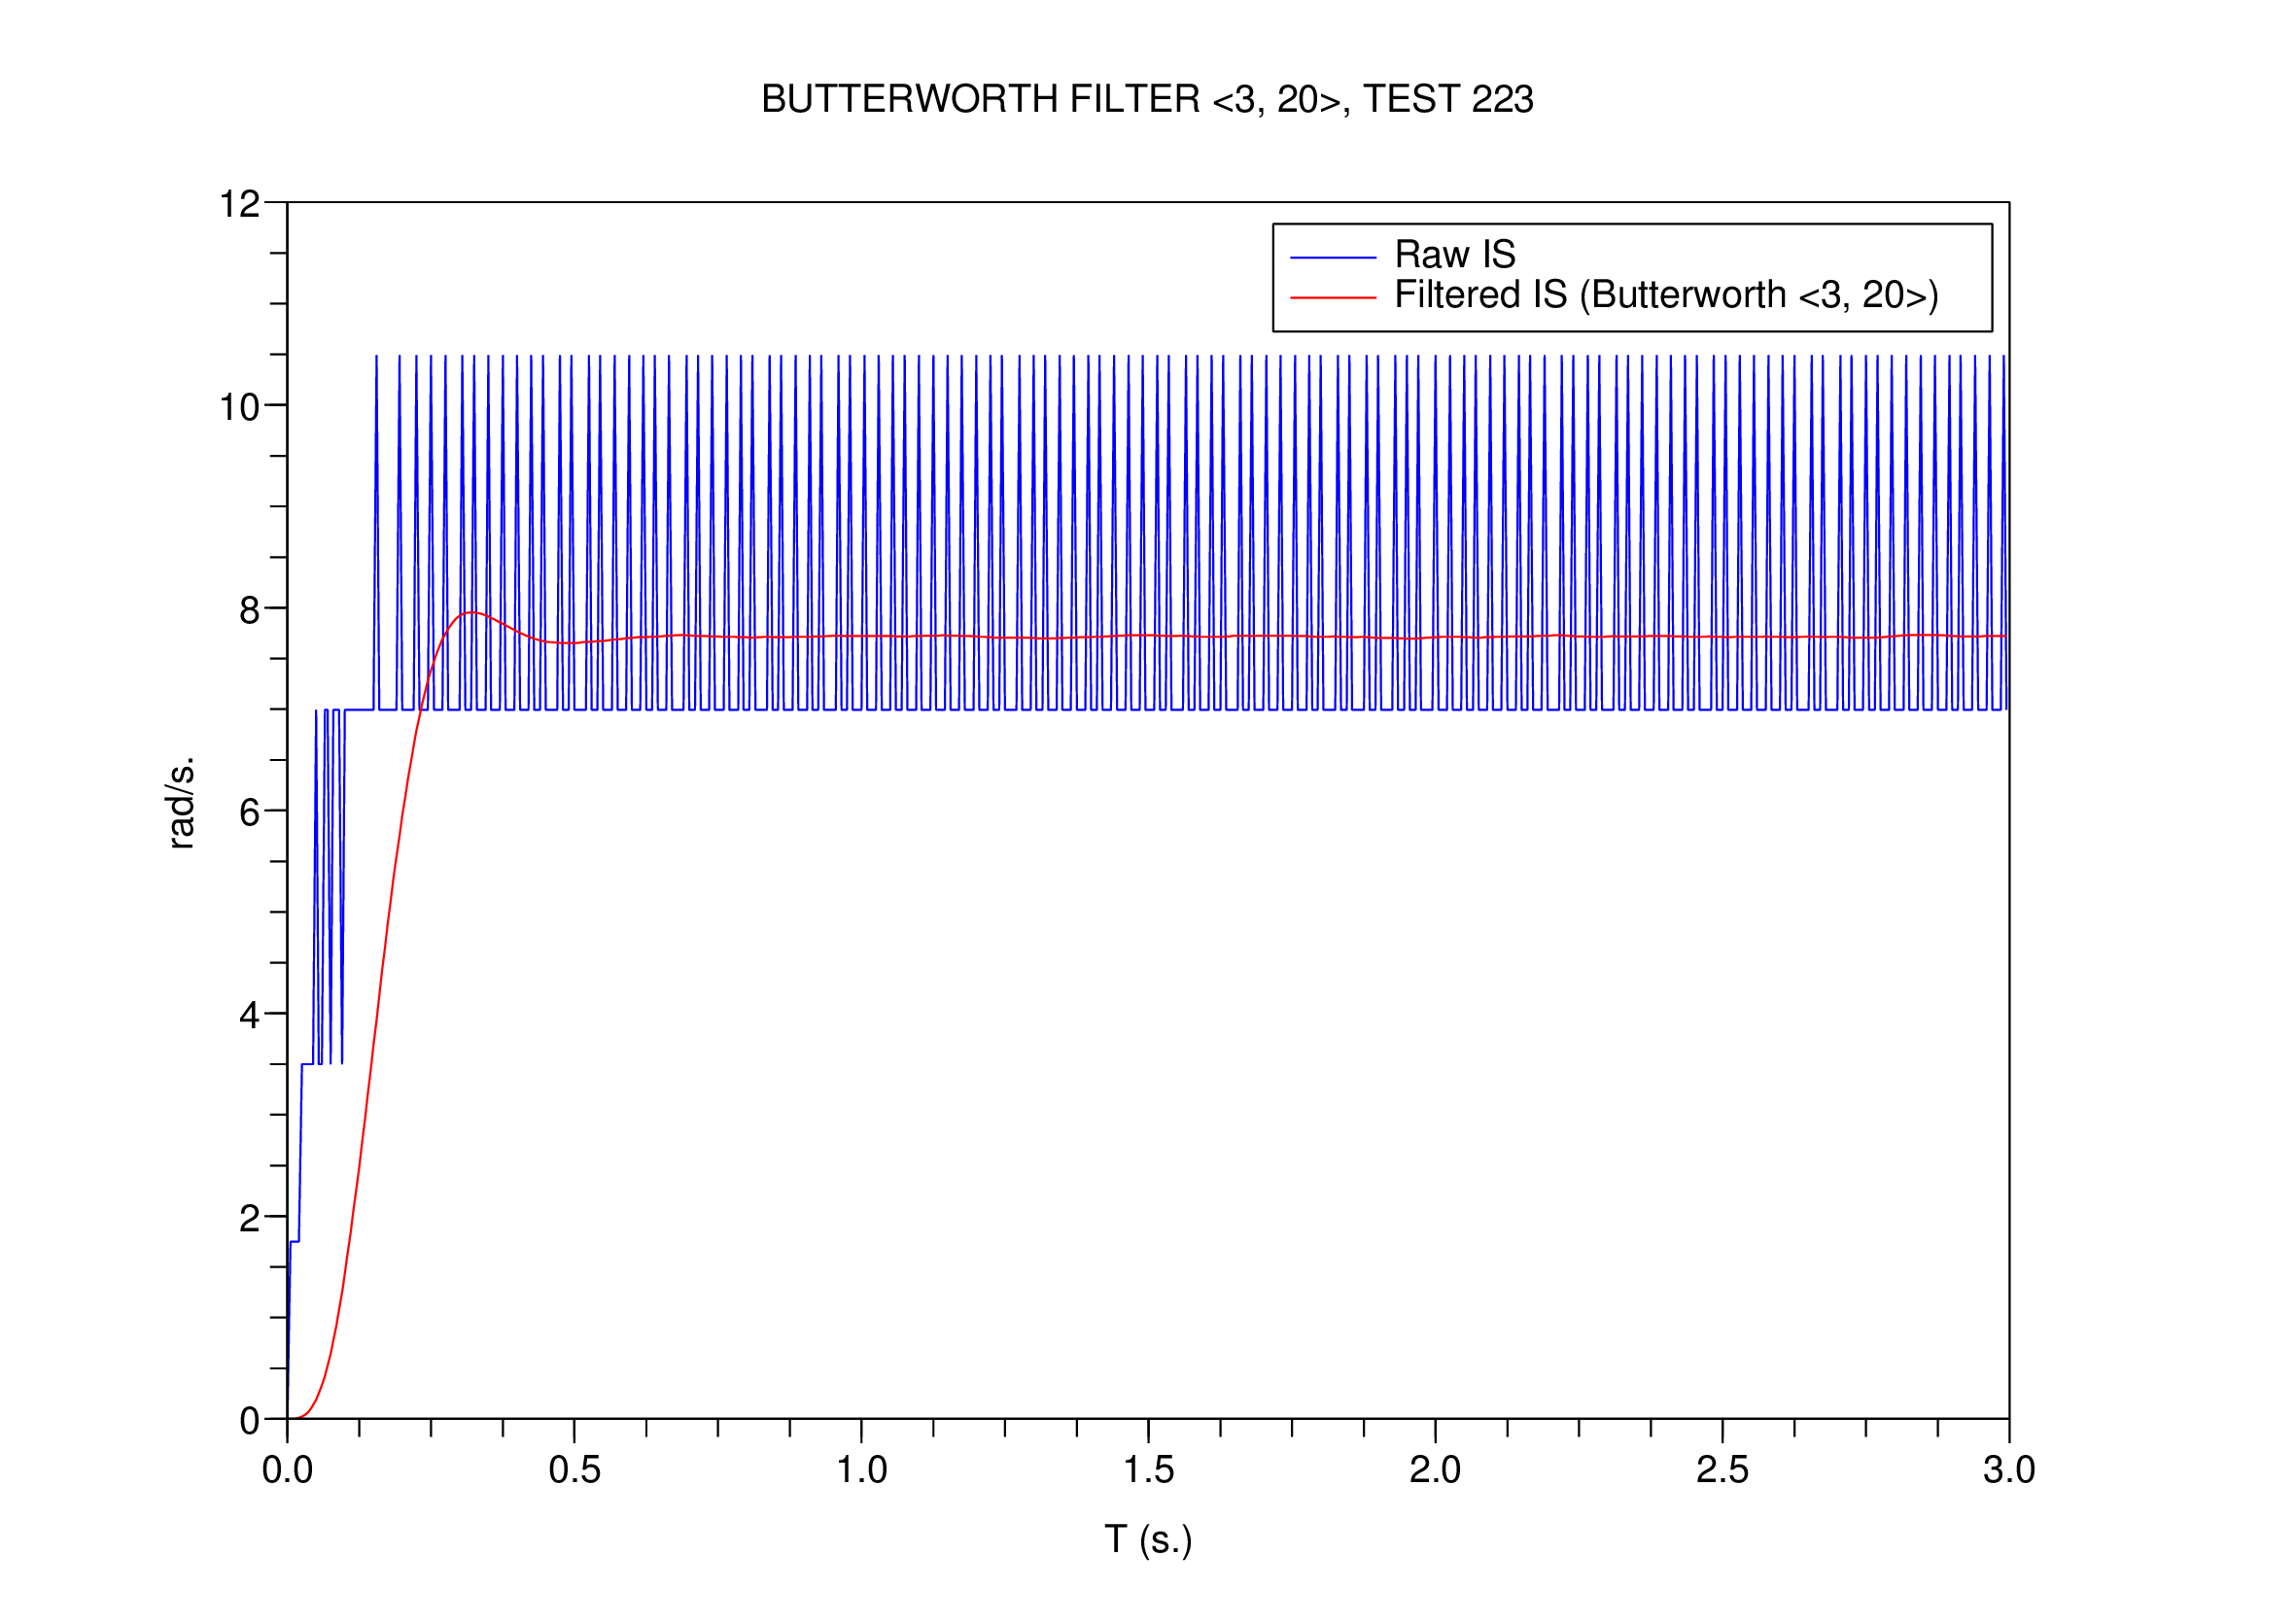
\includegraphics[scale=0.16]{FIGURES_1/butterworth.png}
  \caption[Butterworth Filter]{an example instantaneous speed data filtered with a butterworth operator}
  \label{fig:butterworthResult}
\end{figure}

After some estimations with different cut-off frequencies, we found that a good calibration for this filter is to use an order of $3$ with a cut-off frequency of $20$. Higher cut-off frequencies would have been preferable, so that the over-shoot position could be anticipated, however this configuration introduces also a high degree of spurious noise on the filtered signal that would complicate the next phase of the SOS model parameters identification.

\subsubsection{Filtering Reviewed}

During the second assignment we realized that the estimation of SOS model obtained using the \textbf{butterworth} filter was rather poor, mainly due to the delay in rise and settling time it introduces, and that this problem would have affected the overall project experience if not immediately solved.

As reported at the beginning of the second assignment, we jumped back to the filtering techniques and tried a new approach based on \textbf{cubic splines}, a technique used for interpolation. The advantage of this choice is that now the filtered signal has a slope that is nearly overlapping the experimental data, meaning that it is no longer affected by the delay introduced with butterworth. This increasingly improved our estimation of $\omega_n$. 

As a consequence of this review work, from this point onward all the data, plots and analysis has been consistently corrected to reflect the newly found values. 

%------------------------------------------------------------------------%

\subsubsection{Data analysis and SOS parameters estimation}

As we have previously seen, the transfer function of a Second Order System has the general formulation of equation \ref{eq:responseSOS}:

\[
  y(s) = {{k \over {{s^2 \over {{\omega_n}^2}} + {2s{\xi} \over
        {\omega_n}} + 1}}u\left (s\right )}
\]

where $k$ is the gain, $\xi$ is the damping factor and $\omega_n$ stands for the natural pulsation of the system. These parameters are unknown, but can be computed from the \textit{filtered signal} with a certain degree of confidence. We briefly summarize here the formulas that must be computed in order to proceed with the system identification:

\begin{itemize}
\item \emph{Overshoot}, maximum oscillation in respect to the steady state value:
\[
  O = {{\left \vert {\omega_{max} - \omega\left (\infty \right )}\right
    \vert} \over {\left \vert {\omega \left (0\right ) - \omega \left
          (\infty \right )}\right \vert}}
\]
where $\omega_{max}$ is the maximum oscillation value;
\item
\[
  k = {\omega_{\infty} \over A}
\]
where $\omega_{\infty}$ is the steady state value ($q$) and $A$ is the amplitude of the input step signal (i.e. the power assigned to the motor). This formula derives from the final value theorem of a Laplace transform.
\item \emph{Damping Factor} ($\xi$):
\[
  \xi = {\sqrt{{\ln^2 O} \over {\pi^2 + \ln^2 O}}}
\]
\item The \emph{Settling Time} $T_s$, estimated as the moment from which the filtered signal value does not oscillate more than a percentile $\alpha{}$ ($=5\%$) from its steady state $q$;
\item \emph{Natural Pulsation} ($\omega_n$), which has three possible formulations:
\[
  \omega_n^1 = {{(\log{\alpha{}} - \log{\overline{N}})}\over{(-\xi * T)}}
\]
where \emph{$\overline{N}$} is computed as: 
\[
	\overline{N} = \frac{1}{(1 - \sqrt[2]{1 - \xi^2})}
\]
\[
  \omega_n^2 = \frac{- \log{\frac{\omega_{(t_0 + T)} - \omega_\infty}{\omega_{(t_0)} - \omega_\infty }}}{\xi * T}
\]
\[
  \omega_n^3 = {{\pi} \over {T\sqrt[2]{1-\xi^2}}}
\]
where $\alpha{}$ ($= 5\%$) is the percentile used as a threshold below which the oscillating signal is considered stable, $t_0$ is a certain time instant and $T$ is the period of the oscillations of the system. Note that in our experiment we used $\omega_n^3$, since it has shown itself to result in the most numerically stable estimation of the $\omega_n$ variable.
\end{itemize}

\subsubsection{Error Estimation}

In order to determine with a good approximation the physical parameters of the Second Order System we tried to fit onto the \LEGOMOTOR{}, we selected the $20$ tests with the best SOS models and computed the average of their $\xi$, $\omega_n$ and $k$ estimations.

Here the notion of ``better'' SOS model is strictly connected to the following error estimators:
\begin{itemize}
\item \emph{Integral Squared Error}:
  \[
	ISE = \int_0^T(\omega_m(t)-\omega(t))^2\,dt
  \]
\item \emph{Integral Absolute Error}:
  \[
	IAE = \int_0^T\|\omega_m(t)-\omega(t)\|\,dt
  \]
\item \emph{Integral Time Squared Error}:
  \[
	ITSE = \int_0^Tt(\omega_m(t)-\omega(t))^2\,dt
  \]
\item \emph{Integral Time Absolute Error}:
  \[
	ITAE = \int_0^Tt\|\omega_m(t)-\omega(t)\|\,dt
  \]
\end{itemize}

We have decided to use a modified version of the \emph{ITAE} error estimator to compare our models in which we have added to the denominator the area of the filtered signal. This change allowed us to compare tests taken using input step functions with different power.

We then validated our estimates of such parameters verifying that the \emph{ITAE} error of all the tests was sensibly reduced using the newly estimated parameters. The improvement can be appreciated in figure \ref{fig:Result}, by simply comparing the green line (SOS model with best parameters) to the black line (original SOS model associated to this test data).

\begin{figure}[htbp]
\center
  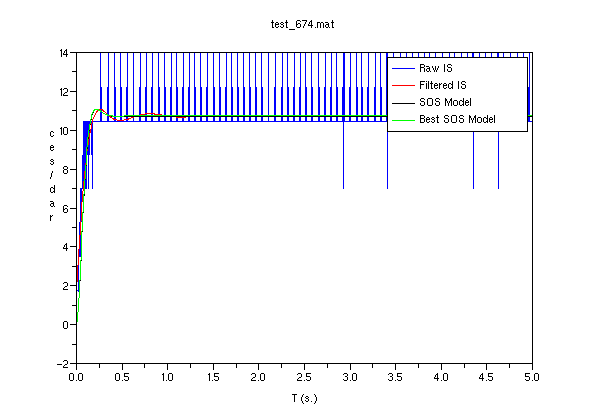
\includegraphics[scale=0.70]{FIGURES_1/power70test24.png}
  \caption{The response of the system: raw instantaneous speed (blue), filtered signal (red), sos model response for current experiment (black), best sos model response (green)}
  \label{fig:Result}
\end{figure}


\subsubsection{Final Results}

In table \ref{tab:results} you can see, for each measured power, the estimations of the four main parameters of our model.  As a consequence of the option \textit{BRAKE = ON}, the steady state value shown in figure \ref{fig:q_avg} grows linearly with the power. The  \textbf{gain}, \textbf{damping factor} and \textbf{natural pulsation} are shown respectively in figures \ref{fig:k_avg}, \ref{fig:csi_avg} and \ref{fig:omega_n_avg}. Note that the ``high'' variance in the estimation of the natural pulsation at very low power inputs could have been lowered by adjusting the \textbf{Cubic Spline} filtering parameters to the different input power levels. This has not been done in the displayed plot to maintain the  homogeneity of the estimated values.

\begin{table*}[htbp]
\centering\small
\parskip=\baselineskip
\begin{tabular}{c|cc|cc|cc|cc}
Power & \multicolumn{2}{c}{Final Value ($q$)} & \multicolumn{2}{c}{Gain ($k$)} & \multicolumn{2}{c}{Damping F. ($\xi$)} & \multicolumn{2}{c}{Nat. Freq. ($\omega_n$)} \\
 $\%$ & avg & $\sigma^2$ & avg & $\sigma^2$ & avg & $\sigma^2$ & avg & $\sigma^2$ \\
\hline
10 & 1.34595 & 5e-05 & 1.81885 & 8e-05 & 0.73356 & 0.002 & 19.88264 & 5 \\
15 & 2.11017 & 3e-05 & 1.90105 & 2e-05 & 0.71283 & 0.0005 & 19.57561 & 0.9 \\
20 & 2.99757 & 3e-05 & 2.02538 & 1e-05 & 0.71225 & 0.0002 & 19.56728 & 0.3 \\
25 & 3.76146 & 5e-05 & 2.03322 & 1e-05 & 0.70605 & 0.0001 & 19.27464 & 0.2 \\
30 & 4.53271 & 4e-05 & 2.04176 & 8e-06 & 0.70764 & 0.0001 & 19.47343 & 0.3 \\
35 & 5.30502 & 3e-05 & 2.04827 & 4e-06 & 0.70973 & 7e-05 & 19.64253 & 0.3 \\
40 & 6.19232 & 0.0009 & 2.09200 & 0.0001 & 0.71359 & 5e-05 & 19.84787 & 0.1 \\
45 & 6.88301 & 0.0002 & 2.06697 & 2e-05 & 0.71315 & 5e-05 & 19.89709 & 0.2 \\
50 & 7.61985 & 0.0001 & 2.05942 & 7e-06 & 0.72138 & 4e-05 & 20.27311 & 0.1 \\
55 & 8.36517 & 4e-05 & 2.05533 & 3e-06 & 0.72404 & 3e-05 & 20.50765 & 0.1 \\
\hline
\end{tabular}
\caption{Estimated parameters of the SOS characterizing the \LEGOMOTOR{} engine.}\label{tab:results}
\end{table*}

From these values we derived our final estimations of the general SOS model characterizing the \LEGOMOTOR{} by applying a simple averaging operation:
\begin{itemize}
	\item $\mathbf{K} = 2.033620$
	\item $\mathbf{\omega_n} = 20.907025$
	\item $\mathbf{\xi} = 0.730782$
\end{itemize}

These values will be at the basis for the next assignment devoted to the design of a \textbf{Controller} for the \LEGOMOTOR{}.

\begin{figure}[htbp]
\center
  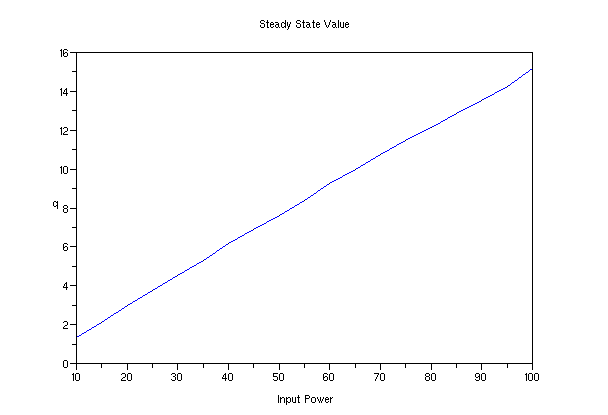
\includegraphics[scale=0.65]{FIGURES_1/steadystatevalue.png}
  \caption{Evolution of steady state value at increasing power}
  \label{fig:q_avg}
\end{figure}

\begin{figure}[htbp]
\center
  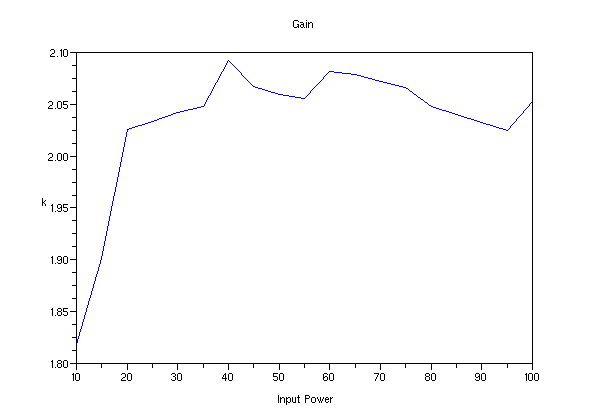
\includegraphics[scale=0.65]{FIGURES_1/Gain.png}
  \caption{Evolution of the Gain value at increasing power}
  \label{fig:k_avg}
\end{figure}

\begin{figure}[htbp]
\center
  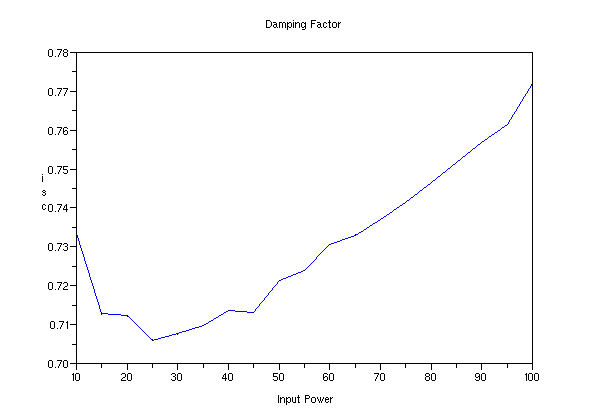
\includegraphics[scale=0.65]{FIGURES_1/DampingFactor.png}
  \caption{Evolution of damping factor value at increasing power}
  \label{fig:csi_avg}
\end{figure}

\begin{figure}[htbp]
\center
  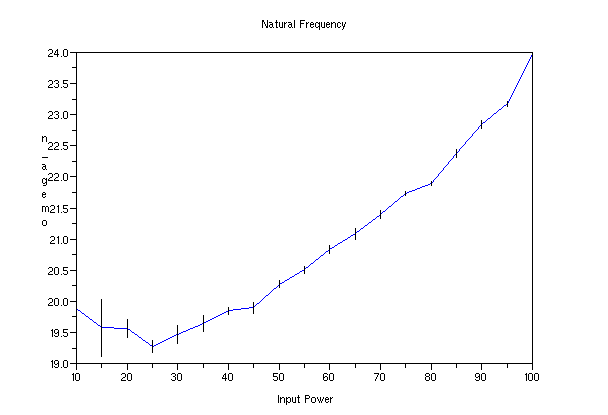
\includegraphics[scale=0.65]{FIGURES_1/NaturalFrequency.png}
  \caption{Evolution of natural frequency value at increasing power}
  \label{fig:omega_n_avg}
\end{figure}

We also tried to plot the frequency response of our SOS model with the aid of \textit{scilab} functions, feeding as input to equation 
\[
  G(s) = {{k \over {{s^2 \over {{\omega_n}^2}} + {2s{\xi} \over
        {\omega_n}} + 1}}}
\]

the parameters identified, for example, with an input step function with power $50\%$, as shown in figure \ref{fig:bode_plot_sos}. The phase correctly decays of $180\deg$ since we have a couple of complex conjugate poles in our model, while the slope of the Magnitude appears to be of nearly $-40 dB$ from $1$ to $10$ Hz. 

\[
p1  = - 15.278478 + 14.271364i  
\]
\[
p2  = - 15.278478 - 14.271364i
\]

\begin{figure}[htbp]
\center
  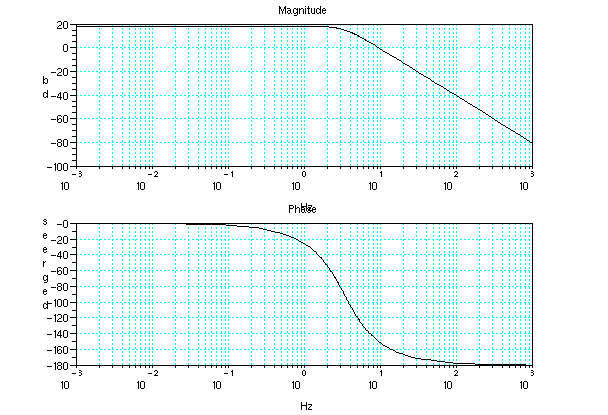
\includegraphics[scale=0.65]{FIGURES_1/BODE_PLOT.png}
  \caption[Bode Plot]{The magnitude and phase of the frequency response given by the parameters identified in the time domain for the input step function with $50\%$ of power.}
  \label{fig:bode_plot_sos}
\end{figure}


%In figure \ref{fig:Result}, it's possible to appreciate the final result of our work:
%\begin{itemize}
%\item \textit{Blue line}: raw instantaneous speed values;
%\item \textit{Red line}: instantaneous speed smoothed with the Butterworth filter;
%\item \textit{Black line}: SOS response signal resulting from the SOS model of the filtered signal;
%\item \textit{Green line}: SOS response signal using the best parameters estimated to be the best;
%\end{itemize}
%-----------------------------------------------%


\subsection{Experiment: Sinusoid Input Function}

In this experiment we decided to use as input function for our \LEGOMOTOR{} a sinusoid signal with different frequency of oscillation and fixed amplitude. The goal of this experiment is determine the frequency response of the \LEGOMOTOR{} engine using a frequency approach.

\subsubsection{Measurements}

For this experiment we modified the code previously written so that it could now support a sinusoidal input signal with arbitrarily chosen amplitude.

In this experiment the data is sampled at intervals of $0.005s (t_{sampling})$, while each test lasts $60s (t_e)$. Therefore by the \emph{Theorem of Nyquist-Shannon} we know that the maximum frequency we can properly sample and reconstruct is given by: 
\[
f_{max} = {1  \over { t_{sampling} \cdot 2} } = 100\: Hz 
\]

Since we experienced a certain degree of numerical instability in our estimation of \textit{magnitude} and \textit{phase}, in the actual case of our measurements we limited our frequency well below this threshold.

We fixed the sinusoid signal amplitude($A$) to $50\%$ of the motor supply power, while we made the frequency vary among several values computed using the following equation:
\[
f ={ (test_{n})^{1.5} \over t_e }
\]
with $f < f_{max} $.

\subsubsection{Data Loading and Filtering}

Similarly to what we have done in the previous experiment with the time domain approach, we load from a file the sampled data of the system response plus the samples of the input signal fed to the system. Again, the space samples are transformed into radians and proportionally redistributed, when necessary. From these data we derive the \textit{Instantaneous Speed}, over which we apply one of our \textit{low pass} filtering techniques to eliminate the high frequencies typical of spurious errors and white noise.

The filters were configured as in the following description:
\begin{itemize}
\item \textbf{Moving Average Filter}, only simple (homogeneously weighted), with a variable window size equal to
\[
	max\Big{(}
	{(N_{samples} \cdot T_{IS}) \over (t_{e} \cdot 10)},\: 3\Big{)}
\]
\item \textbf{Exponential Filter} with a single \textit{forgetting factor} ranging from $0.05$ to $0.4$;
\item \textbf{Double Exponential Filter} with a couple of \textit{forgetting factors}, ranging again in the same discrete set of values;
\item \textbf{Butterworth Filter}, with an order of $3$ and various cut-off frequency values;
\end{itemize}

In this case the filter that had shown to behave better was \textit{Moving Average Filter} since it does not introduce artificial delay in the \textit{phase}, like the \textit{Butterworth Filter}, nor smooth too much the \textit{magnitude} thanks to the self adjusting window size.

In figure \ref{fig:frequencyAvgSin} you can appreciate the result of this filtering operation by looking at the line with red color.

\begin{figure}[htbp]
\center
  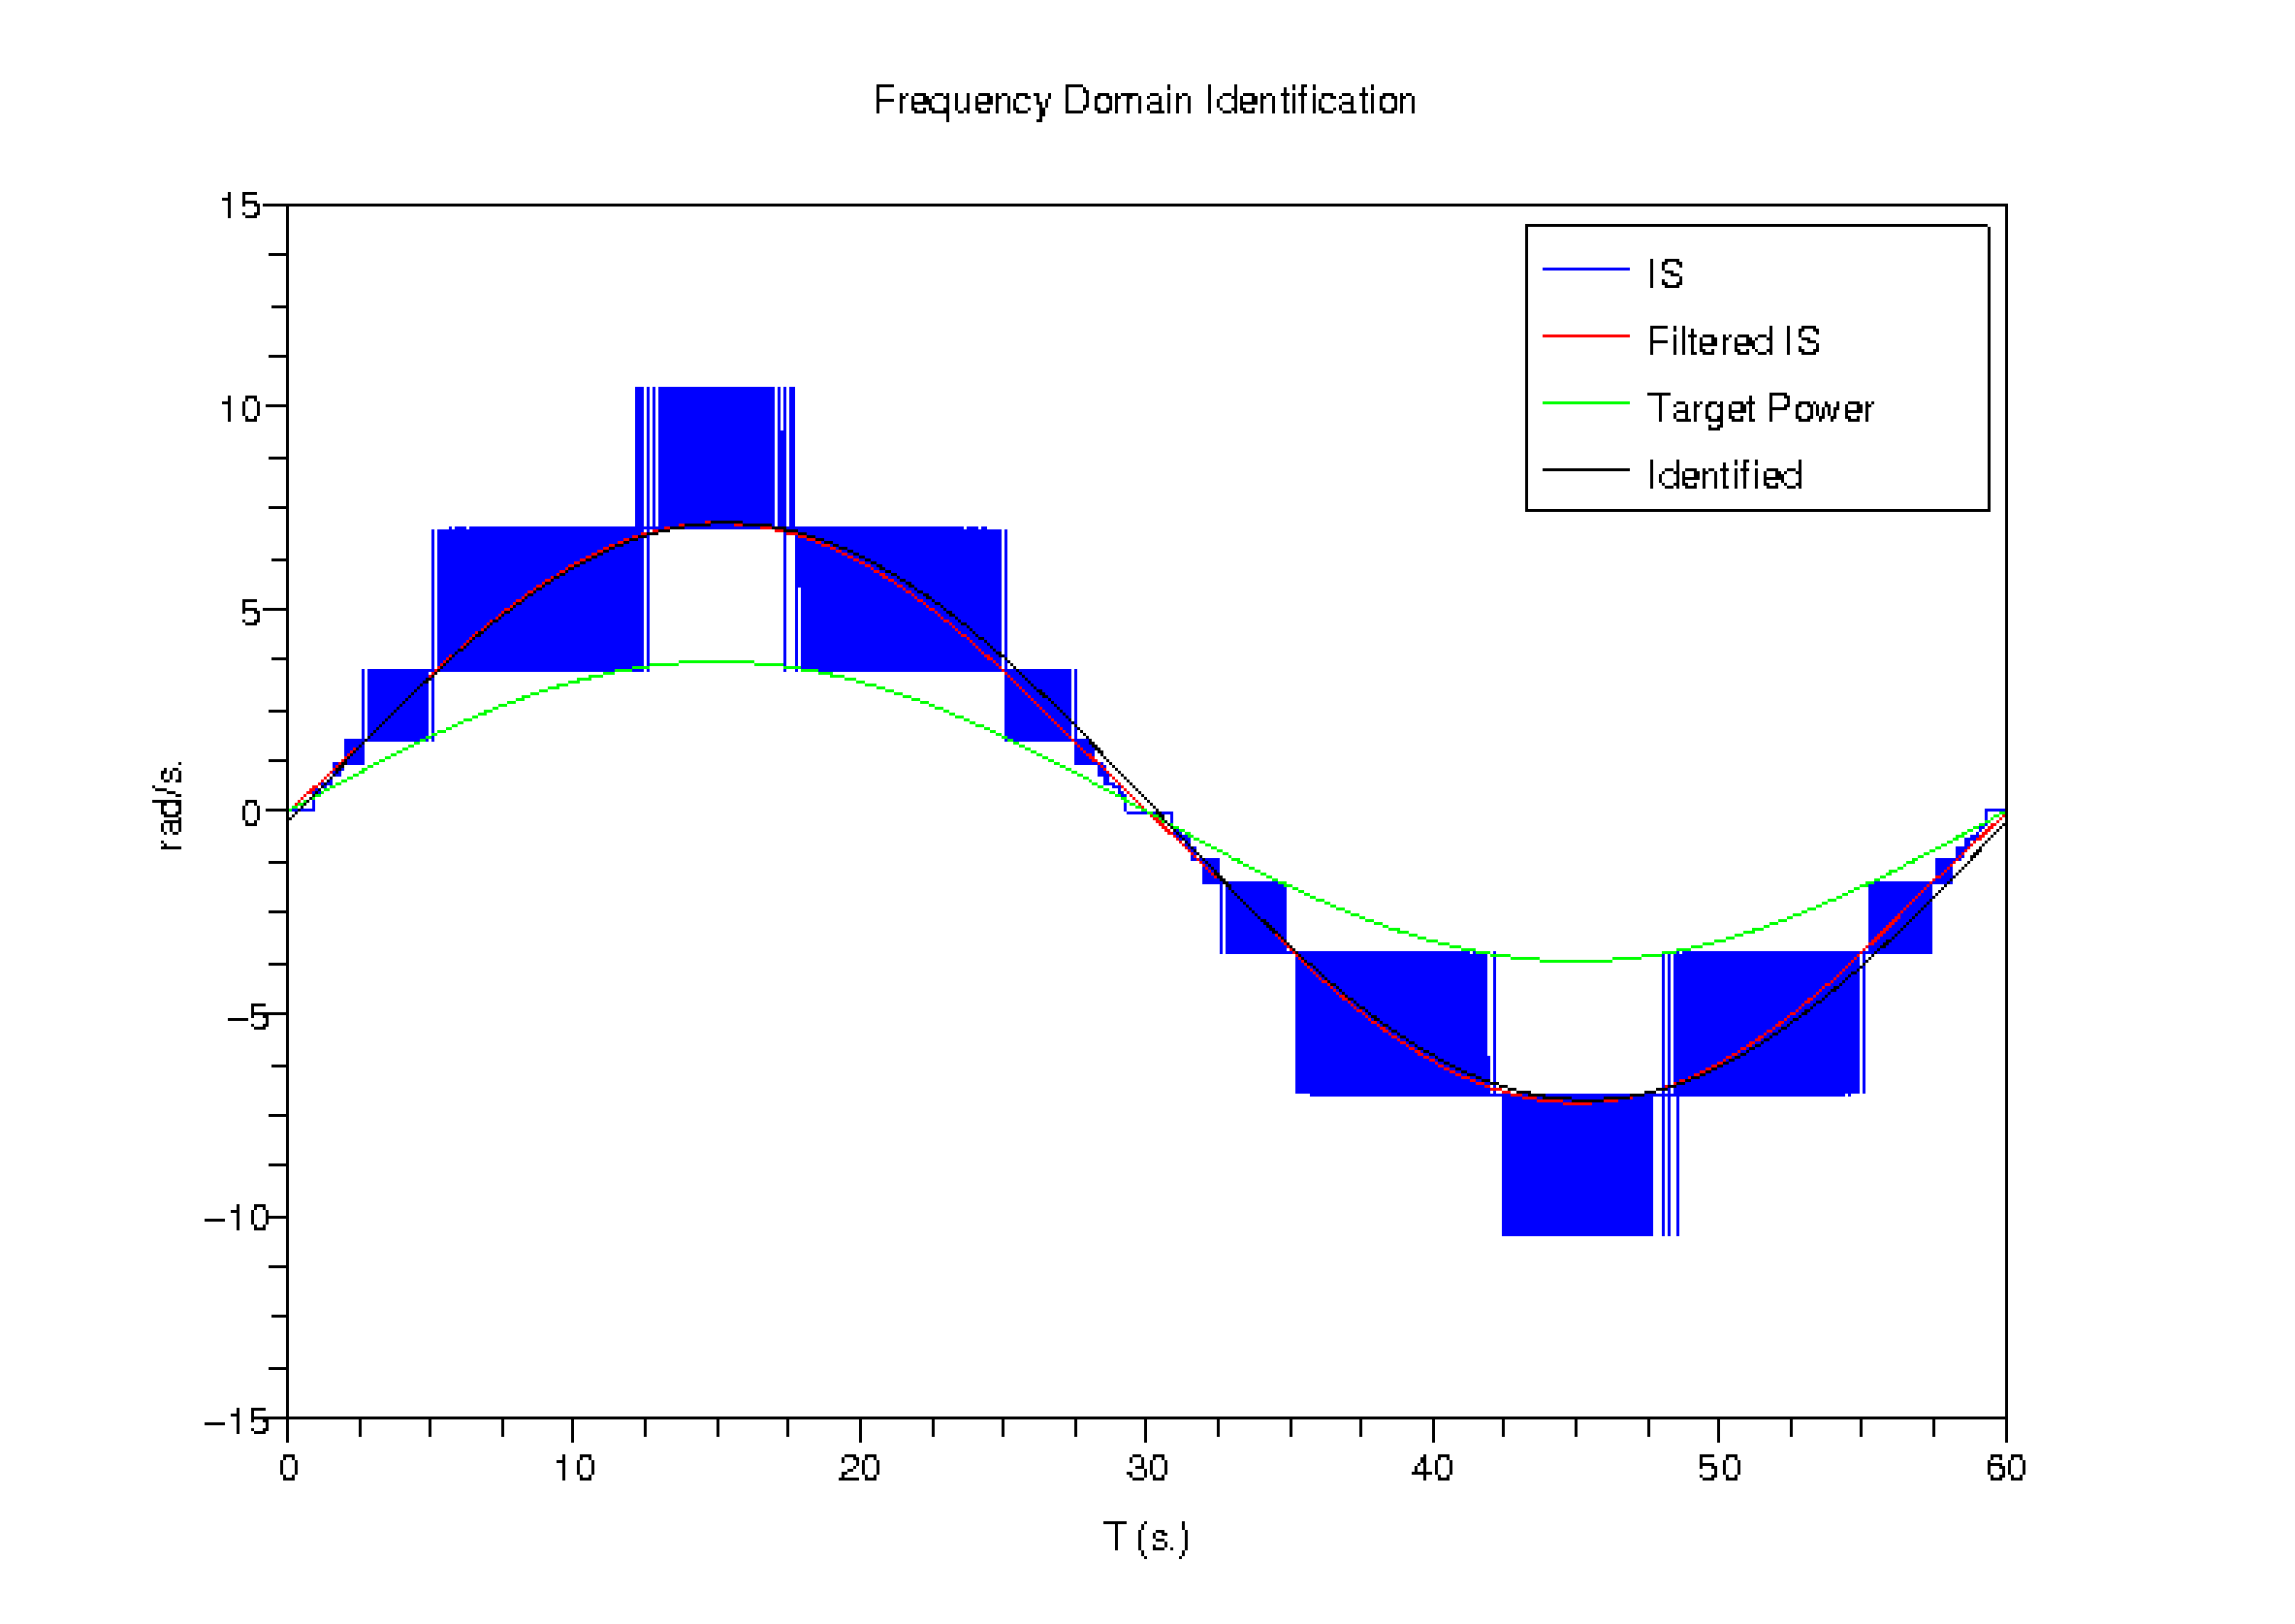
\includegraphics[scale=0.16]{FIGURES_1/frequencyAvgSin.png}
  \caption{The response of the system: raw instantaneous speed (blue), filtered signal (red), reconstructed response signal (black) and best SOS model (green).}
  \label{fig:frequencyAvgSin}
\end{figure}

\subsubsection{Frequency Response Identification}

The identification in the frequency domains proceeds as follows: we feed to our asymptotically linear system $G(j\omega{})$ a sinusoidal function with the general formulation
\[
u(t) = A\small{}\cdot{} sin(\omega{}t)
\]

and obtain an harmonic response of equation
\[
y(t) = \|G(j\omega{})\|A\small{}\cdot{}sin(\omega{}t+\angle{G(j\omega{})})
\]

The \emph{Gain}  is given by the ration between the peaks of the input and those of the outputs:
\[
\|G(j\omega{})\| = \frac{y_{max}}{u_{max}}
\]

The \emph{Phase} is estimated using the peak times $t_y$ and $t_y$ of the output and input signals respectively:
\[
\omega{}t_y + \angle{G(j\omega{})}=\frac{\pi{}}{2} + k_y2\pi{}
\]
\[
\omega{}t_u + \angle{G(j\omega{})}=\frac{\pi{}}{2} + k_u2\pi{}
\]

with $k_y$,$k_u$ 
$\in{} \mathbb{Z}$.

Hence:
\[
\angle{G(j\omega{})}=\omega{}(t_u-t_y) + (k_y-k_u)2\pi{},\; \angle{G(j\omega{})} \in{[-2\pi{},0]}
\]

By collecting samples of data at different input frequencies it's possible to reconstruct the frequency response shape, since it is uniquely characterized by its \textit{magnitude} and \textit{phase} values shown in the \emph{Bode Diagram} \ref{fig:bode_plot}. From the \textit{phase} plot it's possible to see that the \LEGOMOTOR{} engine behaves like a Second Order System because we reach $-180\deg$. Like in the time domain identification, we observe that the slope in the \textit{magnitude} plot has a decay of only $-10\:dB$.

\begin{figure}[htbp]
\center
  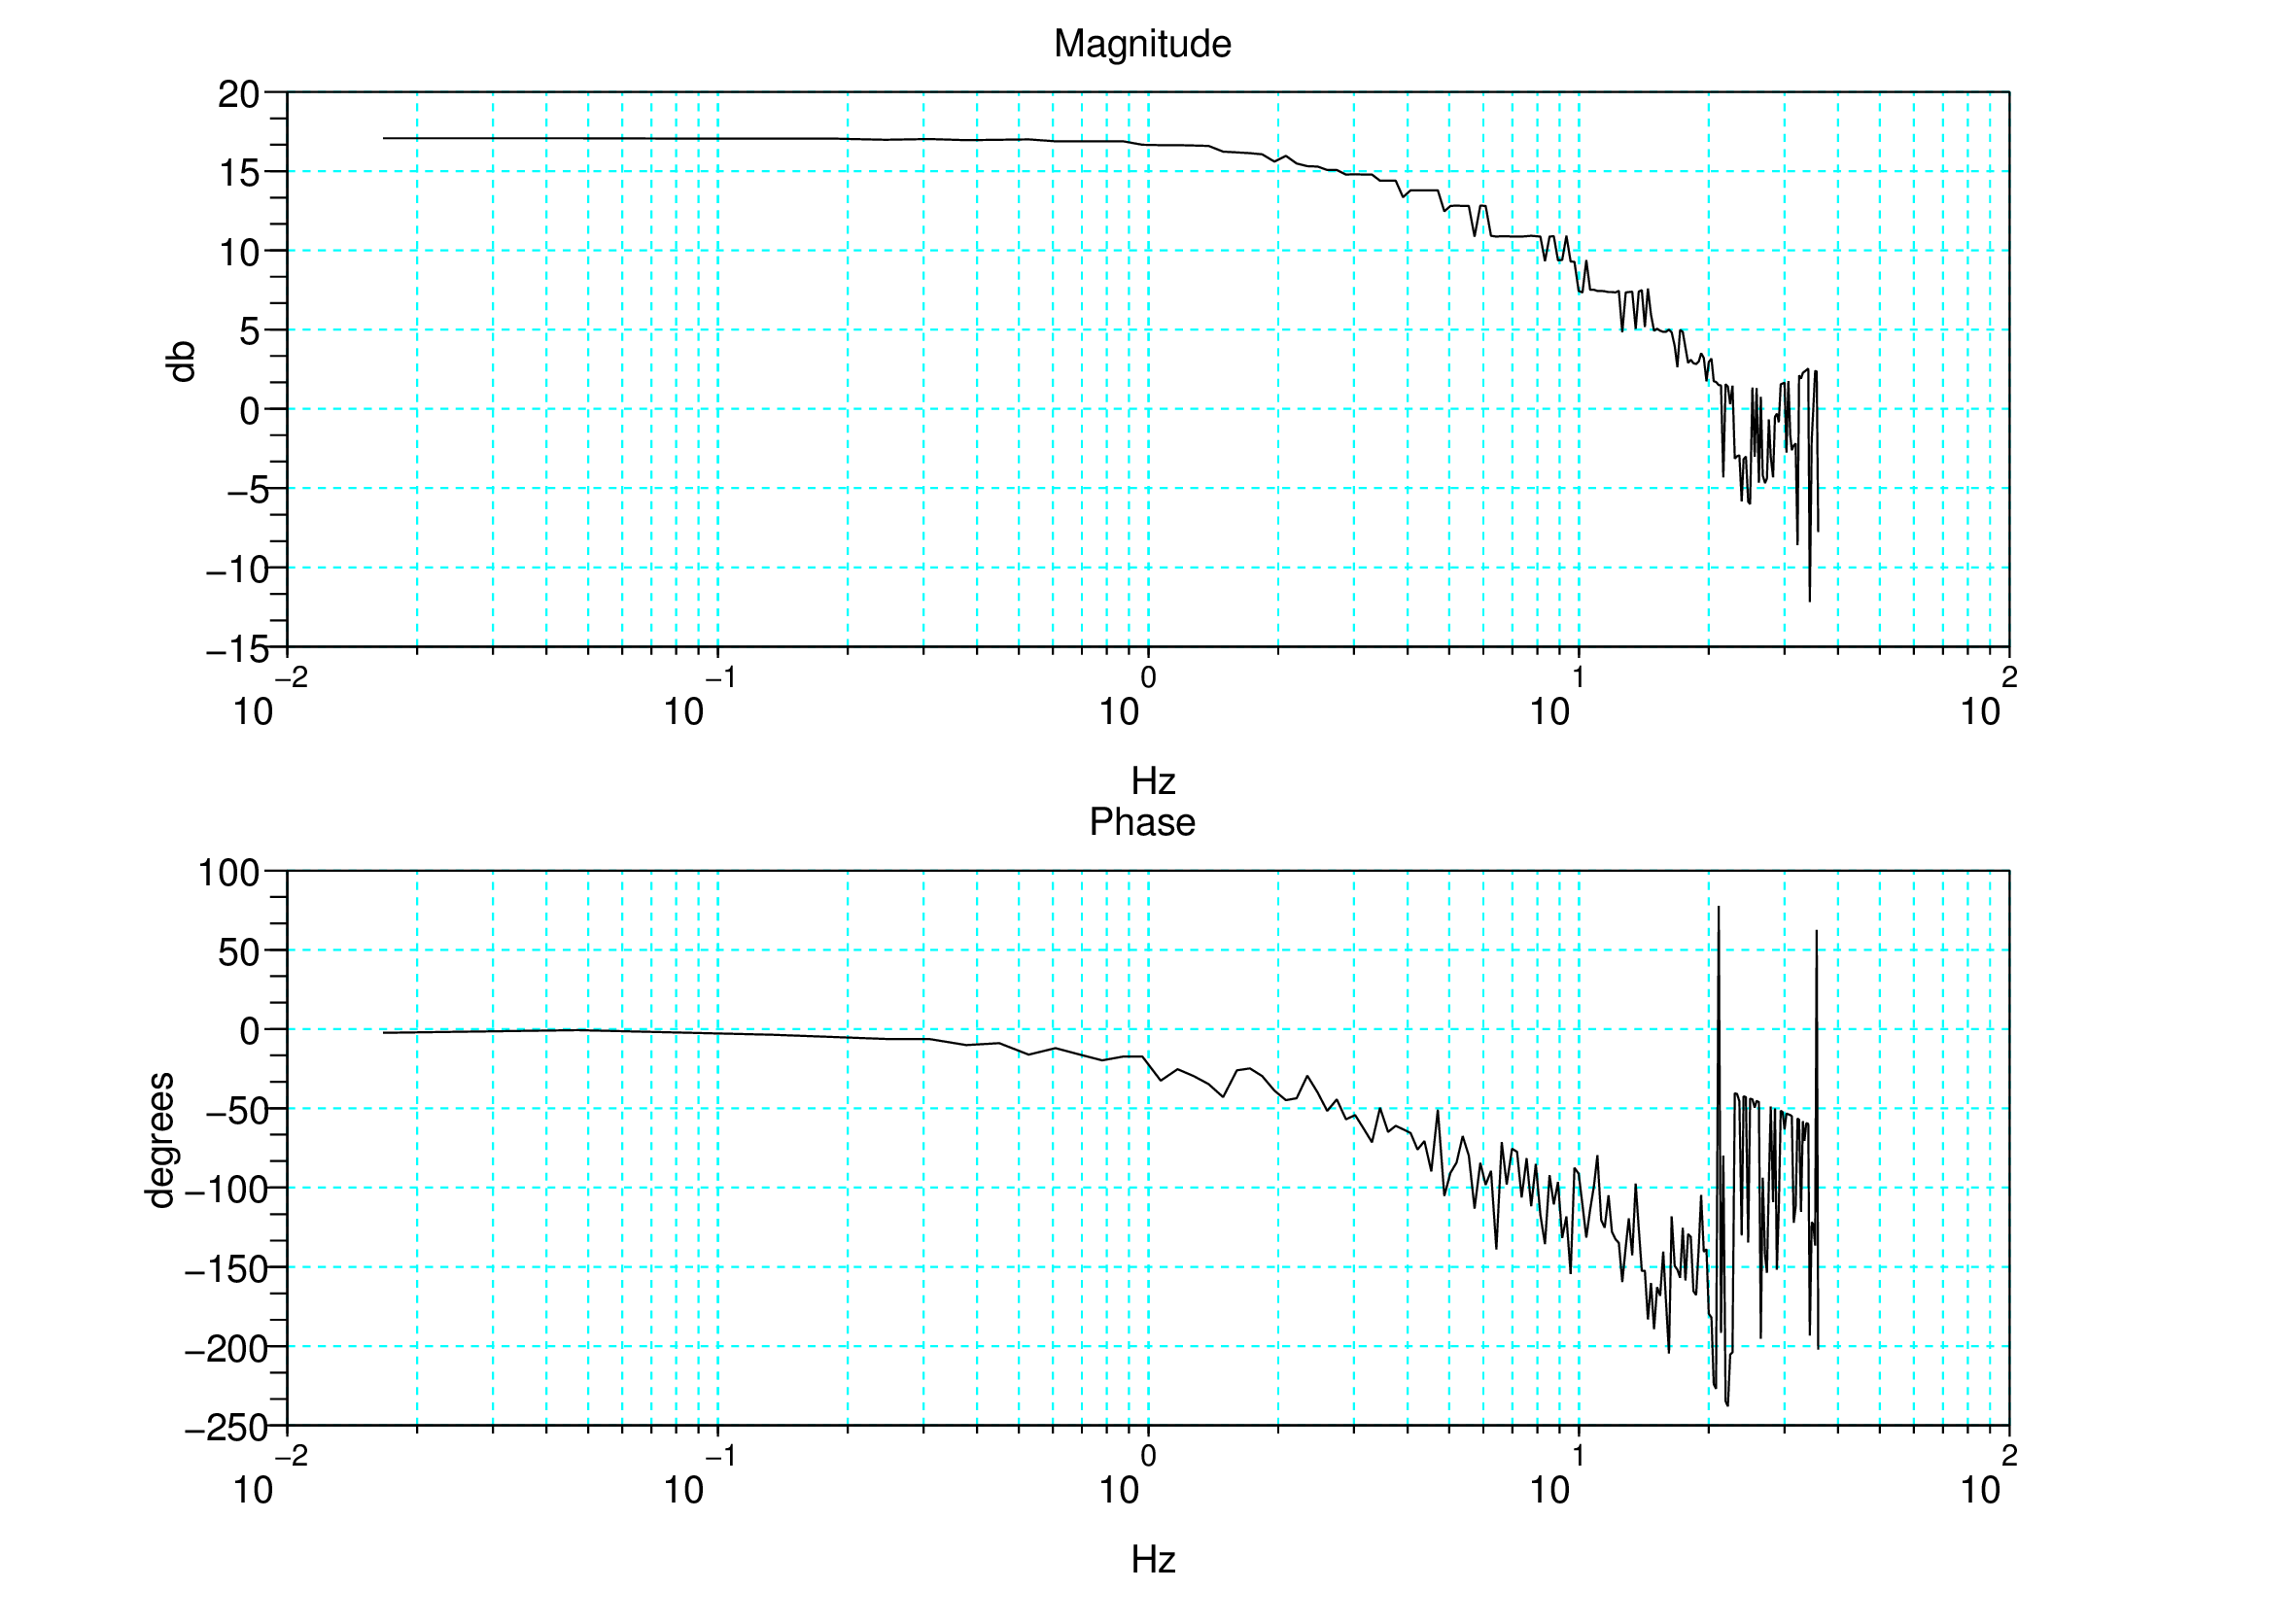
\includegraphics[scale=0.16]{FIGURES_1/bode_plot_sin.png}
  \caption[Bode Plot]{The magnitude and phase of the frequency response given in input a sinusoidal signal with amplitude power $50\%$.}
  \label{fig:bode_plot}
\end{figure}

In the \textit{magnitude} plot we can't see the peak in correspondence to the resonance frequency as we would expect with a Second Order System. This may have been due to the fact the frequencies at which we sample have been selected using a function growing exponentially (with factor $1.5$), so we may have missed to properly sample in the neighbourhood of such frequency. Therefore we have repeated the measurements in the range from $1 Hz$ to $40 Hz$, taking measurements for over $600$ equidistant frequencies. This experiment confirmed the behaviour shown in figure \ref{fig:bode_plot}.